% fig-calplanning: calibration pool planning (2x2 grid)
% Data: R/calplanning_*.csv  →  out/calplanning-panel-[a-d].tex
% Panel letters via \panellabel after \end{axis}; titles centered over plot box.
\documentclass[border=2pt]{standalone}
% inspect_style.tex: Shared style definitions for all Inspect figures
% Enforces uniform fonts, colors, and panel label positioning

\usepackage[T1]{fontenc}
\usepackage{lmodern}  % Latin Modern for Type 1 fonts
\usepackage{amssymb}  % \blacksquare for shared legends
\usepackage{pgfplots}
\usepackage{pgfplotstable}
\pgfplotsset{compat=1.18}

% Color palette (Okabe-Ito colorblind-safe, print-safe)
% -- Backbones (used wherever PatchCore vs Dinomaly are distinguished)
\definecolor{cPatchcore}{HTML}{0072B2}   % blue
\definecolor{cDinomaly}{HTML}{D55E00}    % vermillion
% -- Decision classes / gates
\definecolor{cAccept}{HTML}{009E73}      % green
\definecolor{cDefer}{HTML}{E69F00}       % orange
\definecolor{cReject}{HTML}{D55E00}      % red
\definecolor{cControl}{HTML}{56B4E9}     % light blue
\definecolor{cTransfer}{HTML}{CC79A7}    % pink
% -- Benchmarks (canonical palette; used wherever MVTec/VisA/MPDD are
%    distinguished, so benchmark colouring is uniform across all figures and
%    never collides with the backbone blue/vermillion above)
\definecolor{cMVTecAD}{HTML}{0072B2}     % blue
\definecolor{cVisA}{HTML}{E69F00}        % orange
\definecolor{cMPDD}{HTML}{009E73}        % green

% Typography defaults
\newcommand{\figfont}{\fontsize{8}{9.5}\selectfont}
\newcommand{\axislabelfont}{\fontsize{9}{10}\selectfont}
\newcommand{\titlefont}{\fontsize{9}{10}\selectfont}
\newcommand{\tickfont}{\fontsize{7}{8}\selectfont}
\newcommand{\panellabelfont}{\fontsize{9}{10}\selectfont\bfseries}

% Panel label OUTSIDE the axis (axis clip would otherwise swallow it).
% Usage after \end{axis}: \panellabel{axname}{a}
% Parked in the left gutter at the top of the axis frame — NOT on the
% title baseline — so titles can stay truly centered over the plot box.
\newcommand{\panellabel}[2]{%
  \node[anchor=south east, font=\panellabelfont, inner sep=0.5pt]
    at ([xshift=-8pt, yshift=7pt] #1.north west) {\textbf{#2}};%
}

% Standard axis styles. Titles centered above the plot box only.
\pgfplotsset{
  inspect/centertitle/.style={
    title style={at={(0.5,1.10)}, anchor=south, font=\titlefont},
  },
  inspect default/.style={
    axis x line=bottom,
    axis y line=left,
    xlabel style={font=\axislabelfont},
    ylabel style={font=\axislabelfont},
    inspect/centertitle,
    x tick label style={font=\tickfont},
    y tick label style={font=\tickfont},
    legend style={font=\tickfont, draw=none, fill=none},
  }
}


% cGate is the G1/G2 accept-band colour used only in this figure. Benchmark
% colours (cMVTecAD/cVisA/cMPDD) come from inspect_style.tex so they match the
% rest of the paper.
\definecolor{cGate}{HTML}{0072B2}

\begin{document}
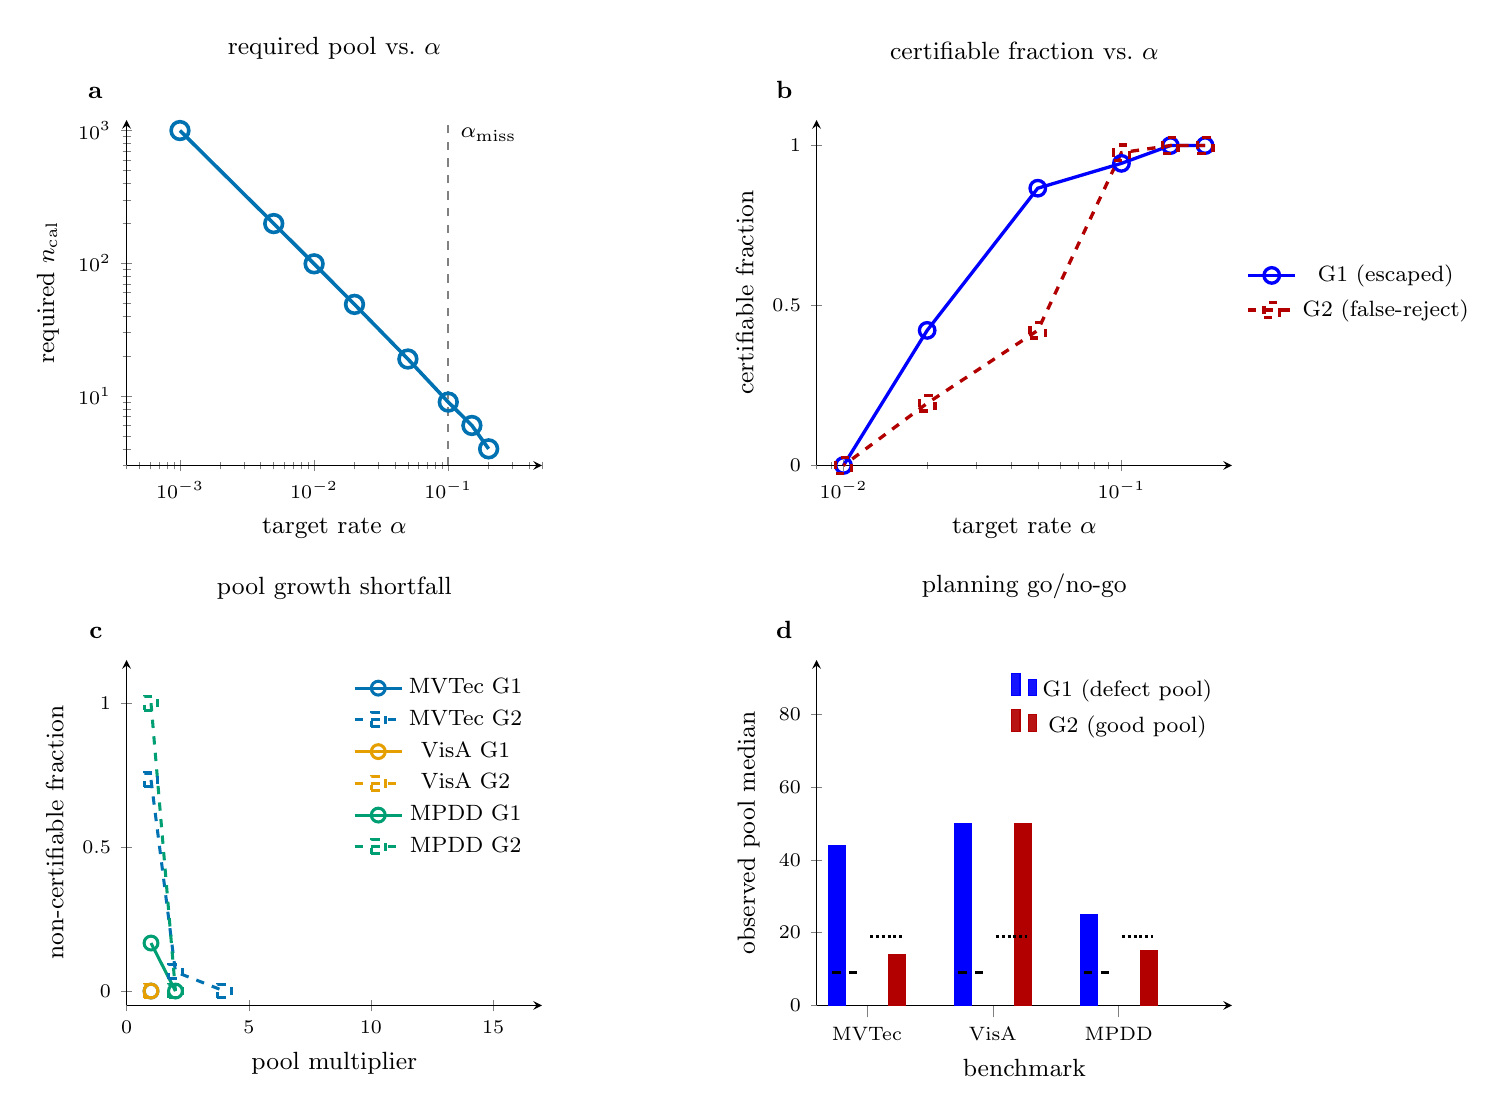
\begin{tikzpicture}[font=\figfont]

% Panels enlarged; legends clear of in-axis series/bars.

% Panel a: requirement curve + observed pools.
% xmin below α=0.001 (full curve inside, clip on). xmax padded so band
% labels fit inside the frame to the right of α_miss — no left spillover,
% no bleed into panel b.
\begin{axis}[
  inspect default,
  name=axa, width=2.70in, height=2.35in, at={(0.40in,2.75in)},
  xmode=log, ymode=log,
  xmin=0.0004, xmax=0.50, ymin=3, ymax=1200,
  clip=false,
  xlabel={target rate $\alpha$},
  ylabel={required $n_{\mathrm{cal}}$},
  % Outside right into the column gutter — in-axis corners all meet the curve/bands.
  legend style={at={(1.02,0.82)}, anchor=west, font=\fontsize{8}{9}\selectfont,
                draw=none, fill=white, fill opacity=0.92, text opacity=1,
                inner sep=2pt, row sep=1pt},
  title={required pool vs.\ $\alpha$},
]
% generated by process_calplanning.R -- panel a
\addplot[cGate, mark=o, line width=1.3pt, mark size=3.2pt, forget plot] coordinates {
  (0.2000,4) (0.1500,6) (0.1000,9) (0.0500,19) (0.0200,49) (0.0100,99) (0.0050,199) (0.0010,999)
};
\draw[gray, dashed, line width=0.8pt] (axis cs:0.1000,3) -- (axis cs:0.1000,1200);
\node[anchor=south west, font=\figfont, text=black] at (axis cs:0.1050,700) {$\alpha_{\mathrm{miss}}$};

\end{axis}
\panellabel{axa}{a}

% Panel b: attainment — every in-axis corner meets a series; park legend
% just outside the right spine (clip=false only for that overhang).
\begin{axis}[
  inspect default,
  name=axb, width=2.70in, height=2.35in, at={(3.85in,2.75in)},
  xmode=log, xmin=0.008, xmax=0.25, ymin=0, ymax=1.08,
  clip=false,
  xlabel={target rate $\alpha$},
  ylabel={certifiable fraction},
  legend style={at={(1.02,0.50)}, anchor=west, font=\fontsize{8.5}{9.5}\selectfont,
                draw=none, fill=white, fill opacity=0.92, text opacity=1,
                inner sep=2pt, row sep=1pt},
  title={certifiable fraction vs.\ $\alpha$},
]
% generated by process_calplanning.R -- panel b
\addplot[blue, mark=o, line width=1.2pt, mark size=2.8pt] coordinates {(0.2000,1.0000) (0.1500,1.0000) (0.1000,0.9444) (0.0500,0.8667) (0.0200,0.4222) (0.0100,0.0000)};
\addlegendentry{G1 (escaped)}
\addplot[red!70!black, mark=square, dashed, line width=1.2pt, mark size=2.8pt] coordinates {(0.2000,1.0000) (0.1500,1.0000) (0.1000,0.9778) (0.0500,0.4222) (0.0200,0.1944) (0.0100,0.0000)};
\addlegendentry{G2 (false-reject)}

\end{axis}
\panellabel{axb}{b}

% Panel c: shortfall — series are truncated after first zero (see R emitter),
% so the right half stays empty for the legend.
\begin{axis}[
  inspect default,
  name=axc, width=2.70in, height=2.35in, at={(0.40in,0.05in)},
  xmin=0, xmax=17, ymin=-0.05, ymax=1.15,
  xlabel={pool multiplier},
  ylabel={non-certifiable fraction},
  legend style={at={(0.98,0.98)}, anchor=north east, font=\fontsize{8}{9}\selectfont,
                draw=none, fill=white, fill opacity=0.92, text opacity=1,
                legend columns=1, inner sep=2pt, row sep=0.5pt},
  title={pool growth shortfall},
]
% generated by process_calplanning.R -- panel c (non-certifiable)
\addplot[cMVTecAD, mark=o, line width=1.1pt, mark size=2.5pt] coordinates {(1,0.0000)};
\addlegendentry{MVTec G1}
\addplot[cMVTecAD, mark=square, line width=1.1pt, mark size=2.5pt, dashed] coordinates {(1,0.7333) (2,0.0667) (4,0.0000)};
\addlegendentry{MVTec G2}
\addplot[cVisA, mark=o, line width=1.1pt, mark size=2.5pt] coordinates {(1,0.0000)};
\addlegendentry{VisA G1}
\addplot[cVisA, mark=square, line width=1.1pt, mark size=2.5pt, dashed] coordinates {(1,0.0000)};
\addlegendentry{VisA G2}
\addplot[cMPDD, mark=o, line width=1.1pt, mark size=2.5pt] coordinates {(1,0.1667) (2,0.0000)};
\addlegendentry{MPDD G1}
\addplot[cMPDD, mark=square, line width=1.1pt, mark size=2.5pt, dashed] coordinates {(1,1.0000) (2,0.0000)};
\addlegendentry{MPDD G2}

\end{axis}
\panellabel{axc}{c}

% Panel d: planning bars — legend NE above bar headroom.
\begin{axis}[
  inspect default,
  name=axd, width=2.70in, height=2.35in, at={(3.85in,0.05in)},
  ybar=2pt, bar width=6pt,
  xmin=-0.8, xmax=5.8, ymin=0, ymax=95,
  xlabel={benchmark},
  ylabel={observed pool median},
  xtick={0,2,4}, xticklabels={MVTec, VisA, MPDD},
  legend style={at={(0.98,0.98)}, anchor=north east, font=\fontsize{8.5}{9.5}\selectfont,
                draw=none, fill=white, fill opacity=0.92, text opacity=1,
                inner sep=2pt, row sep=1pt},
  title={planning go/no-go},
]
% generated by process_calplanning.R -- panel d
\addplot[blue, fill=blue] coordinates {(-0.3000,44.0000) (1.7000,50.0000) (3.7000,25.0000)};
\addlegendentry{G1 (defect pool)}
\addplot[red!70!black, fill=red!70!black] coordinates {(0.3000,14.0000) (2.3000,50.0000) (4.3000,15.0000)};
\addlegendentry{G2 (good pool)}
\draw[black, dashed, line width=1.1pt] (axis cs:-0.5500,9.0000) -- (axis cs:-0.0500,9.0000);
\draw[black, densely dotted, line width=1.1pt] (axis cs:0.0500,19.0000) -- (axis cs:0.5500,19.0000);
\draw[black, dashed, line width=1.1pt] (axis cs:1.4500,9.0000) -- (axis cs:1.9500,9.0000);
\draw[black, densely dotted, line width=1.1pt] (axis cs:2.0500,19.0000) -- (axis cs:2.5500,19.0000);
\draw[black, dashed, line width=1.1pt] (axis cs:3.4500,9.0000) -- (axis cs:3.9500,9.0000);
\draw[black, densely dotted, line width=1.1pt] (axis cs:4.0500,19.0000) -- (axis cs:4.5500,19.0000);

\end{axis}
\panellabel{axd}{d}

\end{tikzpicture}
\end{document}
